%\documentclass{jpsj3}
\documentclass[fp,twocolumn]{jpsj3}
%\documentclass[letter,twocolumn]{jpsj3}
%\documentclass[letterpaper,twocolumn]{jpsj3}
\usepackage{txfonts}
\usepackage{algorithm}
\usepackage{algorithmic}
\usepackage{amsmath}
\usepackage{multirow}

\makeatletter
\@dblfptop 0pt
\makeatother

\renewcommand{\topfraction}{.85}
\renewcommand{\bottomfraction}{.60}
\renewcommand{\textfraction}{.15}
\renewcommand{\floatpagefraction}{.6}

\title{Derivaton of the QUBO formulation for sparse estimation}

\author{Tomohiro Yokota$^1$%\thanks{jpsj{\_}edit@jps.or.jp}
  , Makiko Konoshima$^2$, Hirotaka Tamura$^2$, Jun Ohkubo$^3$}
\inst{$^1$Graduate School of Science and Enginnering, Saitama University,
  255 Shimo-Okubo, Sakura-ku, Saitama-shi, 338-8570, Japan\\
  $^2$Fujitsu Laboratories Ltd.,
  4-1-1 Kawasaki, Kanagawa 211-8558, Japan
  $^3$JST, PREST, 4-1-8 Honcho, Kawaguchi, Saitama 332-0012, Japan} %\\

\abst{%In recent years, annealing machine have been developed, and their use methods are considered in fields such as optimization problems and machine learning. In the annealing machine, it is necessary to express the problem to be dealt with in QUBO(Quadratic Unconstrained Binary Optimization) formulation and implement it as hardware. However, since the general method of rewriting to the QUBO format is not known yet, it needs to be derived individually. In this paper, we derive the QUBO formulation for the l1-norm (absolute value function) used in sparse estimation. As a result of experiment, it was possible to predict that one variable could be reduced from the result of numerical experiment by applying the Legendre transformation and Wolf-duality theorem to l1norm. By reviewing the formulation we were actually able to reduce one variable.

l1-normのQUBO形式での定式化を提案する. これにより, スパース推定に対するQUBO形式を導出することができるようになる. Sato et al.(2019)が提案したReLUタイプ関数の定式化の方法を応用することで, l1-normのQUBO形式での導出を行なった. 加えて, 数値実験を通して, 定式を見直すことにより変数を減らすことができた. 
}

%%% Keywords are not needed any longer. %%%
%%% \kword{keyword1, keyword2, keyword3, \1dots} 
%%%

\begin{document}
\maketitle

\section{Introduction}
近年では, D-Wave Systems Inc.のD-Waveや富士通のデジタルアニーラのようなイジング型マシンの開発が進められている. 利用できる量子ビット数が年々増加しており, これにより大きな組み合わせ最適化問題に対してイジング型マシンでの計算ができるようになった. しかし, イジング型マシンで最適化問題を計算するためには, コスト関数をQUBO形式に変換しハードウェアとして実装する必要があるが, QUBO形式への系統的な導出方法はまだ見つかっていない. 

先行研究ではq-loss関数とReLUタイプ関数のQUBO形式での導出がされている. q-loss関数の導出法についてはLegendre変換を適用することでQUBO形式を導出することができた. しかし, ReLUタイプ関数に対しては, Legendre変換だけを適用しただけではコスト関数のmin関数にマイナス符号がついてまう. これによりReLUタイプ関数を他のコスト関数を組み合わせて最適化問題を解くことが困難になる. そこで, Wolfeの双対定理を追加で適用することでこの問題を解決した. 

本稿で紹介するl1-normはスパース推定を行う際に利用されている. スパース推定はデータ解析や画像処理の分野で利用されている. データ解析で利用されるもので代表的なものにLassoがあり, 最小二乗法のコスト関数にl1-normを加えることでスパースな推定を行うことを可能にしている. スパース推定の考え方は, ブラックホールの解析でも利用されている. ブラックホールとても小さく, 今までの手法では解像度が低いため観測することが不可能であった. そこで, 世界中の電波望遠鏡から同時に測定を行い, その観測データに対してスパース推定を行うことで本質的な情報のみを取り出しブラックホールの画像化を行なった. このように, スパース推定をイジング型マシンで行う上でこの研究は重要である.

本稿ではl1-normのQUBO形式での定式化を行う. そのために, Legendre変換およびWolfeの双対定理を用いる. さらに, 定式化を見直すことで, 単純に適用した場合よりも変数を減らせることが確認できた. これはイジング型マシンの量子ビット数に制限がある現在において, ハードウェアへの実装を考える上で重要なことである. 

本稿の構成は次のようになる. 第二章では, QUBO形式, 先行研究, 導出に利用する定理についての説明を行う. 第三章では, l1-normのQUBO形式での導出およびその検証を行う. 第四章では, 

\section{Background}
In this section, we describes the knowledge.

\subsection{QUBO and Ising model} %QUBOとIsingモデルについての説明
Since the QUBO formulation and the Ising model are equivalent, we can be converted to other form if we can be represented one side. The Ising model is represented as follows:
\begin{eqnarray}
  H=-\sum_{i,j}{J_{i,j}\sigma_{i}\sigma_{j}}-\sum_{i}{h_{i}\sigma_{i}}
\end{eqnarray}
where $\sigma_{i}\in \{-1,+1\}$is a spin variable for $i$-th spin, $J_{ij}\in \mathbb{R}$ a quadratic term of $i$ and $j$, and $h_{i}\in \mathbb{R}$ a liner term of $i$. We can easily converted the Ising model to QUBO formulation, which uses binary variable $q_{i}\in \{0,1\}$, by applying $q_{i}=\frac{\sigma_{i}+1}{2}$ and QUBO formulation is represented as follows:
\begin{eqnarray}
  H=-\sum_{i,j}{\tilde{J}_{i,j}q_{i}q_{j}}-\sum_{i}{\tilde{h}_{i}\sigma_{i}}
\end{eqnarray}

\subsection{previous research}
この節では先行研究で行われたq-loss関数とReLUタイプ関数のQUBO形式について記載する.

q-loss関数のコスト関数は次のように表される.
\begin{eqnarray}
  L_{q}(m)=\min{[(1-q)^{2}, (\max{[0,1-m]})^{2}]} \label{q-loss_function}
\end{eqnarray}
ここで, $q\in (\infty,0]$はパラメータであり, $m$は実変数である. 式(\ref{q-loss_function})に対してLegendre変換を適用することで次のように変換できる.
\begin{eqnarray}
  L_{q}(m)=\min_{t}{\left\{(m-t)^{2}+(1-q)^{2}\frac{(1-\text{sign}(t-1))}{2}\right\}} \label{q-loss_function_legendre}
\end{eqnarray}

ReLUタイプ関数のコスト関数は次のように表される.
\begin{eqnarray}
  f(m)=-\min{(0,m)} \label{ReLU_function}
\end{eqnarray}
式(\ref{ReLU_function})に対してLegendre変換を適用することで次のように変換できる.
\begin{eqnarray}
  f(m)=-\min_{t}{\{-mt\}} \quad \text{subject to} \quad -1\leq t\leq 0 \label{ReLU_function_legendre}
\end{eqnarray}
ここで, 式(\ref{ReLU_function_legendre})の$\min$関数にマイナス符号が付いているため, 複数のコスト関数と組み合わせた最適化問題を解くこと困難である. そこで, 式(\ref{ReLU_function_lengendre})に対して, Wolfeの双対定理を適用する. wolfeの双対定理の詳細については次の節で説明を行う.
\begin{eqnarray}
  f(m)=\min_{t,z_{1},z_{2}}{\{mt+z_{1}(t+1)-z_{2}t-M(-m-z_{1}+z_{2})^{2}\}} \label{ReLU_function_wolfe}
\end{eqnarray}
ここで, $M$は大きな正の定数である.
式(\ref{q-loss_function_legendre}),(\ref{ReLU_function_wolfe})について, 二進数展開をすることでQUBO形式を導出することができる.

\subsection{Wolfe-duality} \label{sec:wolfe}
Wolfeの双対定理は不等式制約を持つ最大化問題となる双対問題を導出することができる. 次のような制約を持つ最適化問題を考える.
\begin{equation}
  \left\{
  \begin{aligned}
    & \text{minimize}_{x}  \quad  f_{W}(x) \quad (x\in\mathbb{R}^{n}),\\
    & \text{subject to}  \ \quad h_{i}(x)\leq 0 \quad (i=1,2,\dots,l). \label{object_function}
  \end{aligned}
  \right.
\end{equation}
ここで$f_{W}(x)$の最適化したいある凸関数であり, $h_{i}$は凸な不等式制約である. 最適化問題のラグランジュ関数は次のように表される.
\begin{eqnarray}
  L(x,z)=f_{W}(x)+z^{T}h(x),
\end{eqnarray}
ここで$z$はラグランジュ係数のベクトルである. このとき, Wolfeの双対定理により式(\ref{object_function})の最適化問題は次の最大化問題と等価である.
\begin{equation}
  \left\{
  \begin{aligned}
    & \text{maximize}_{x,z}  \quad L(x,z) \quad ((x,z)\in \mathbb{R}^{n}\times\mathbb{R}^{l}),\\
    & \text{subject to}  \qquad \nabla L(x,z)=0 \ (z \geq 0).
  \end{aligned}
  \right.
\end{equation}
上記に示すように, Wolfeの双対定理は最適化問題を最大化問題に変換する. 

\section{Naive derivation of QUBO formulation for $\ell{l}_{1}$-norm}
この章では絶対値関数のQUBO形式での定式化を行う.
\ref{sec:wolfe}章で説明したWolfeの双対定理を式(\ref{})
\subsection{QUBO formulation}
絶対値関数$f(m)$は次のように定義される.
\begin{eqnarray}
  f(m)=-\min{\{-m,m\}} \label{l1-norm}
\end{eqnarray}
\begin{figure}[htbp]
  \begin{center}
    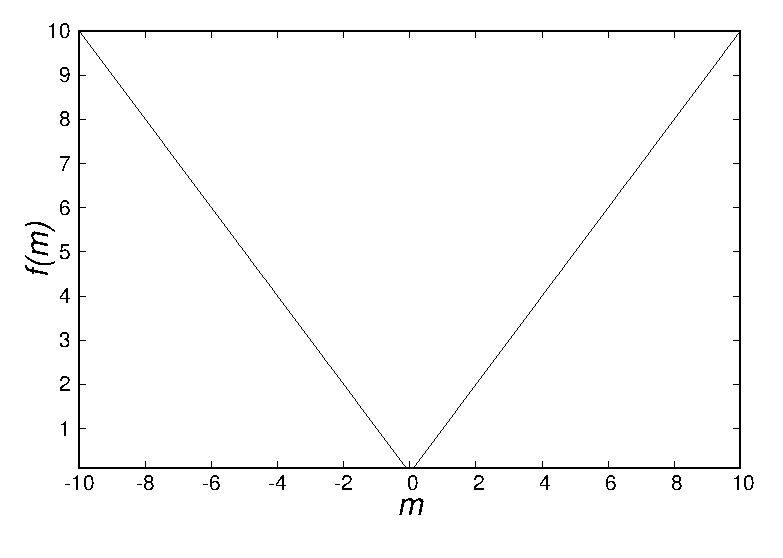
\includegraphics[keepaspectratio,scale=0.50]{absolute.eps}
    \caption{Outline of l1-norm}
    \label{fig:absolute}
  \end{center}
\end{figure}
$f(m)$の概形は図(\ref{fig:absolute})のようになる. また, 式(\ref{l1-norm})に対してLegendre変換を行うと次のように変換できる. 
\begin{eqnarray}
  F(m)=-\min_{t}{\{-mt\}} \quad \text{subject to} \quad \-1 \leq t \leq 1 \label{legendre}
\end{eqnarray}
We could express the quadratic form of $f(m)$ as (\ref{legendre}), but there is the min function is proceded by a minus sign, which makes it difficult to solve an optimization problem that combines multiple cost functions. Let the other cost function be $C(m)$, and the combination with $F(m)$ is as follows:
\begin{eqnarray}
  \min_{m}{\{C(m)+F(m)\}} &=& \min_{m}\left\{C(m)-\min_{t}{\{-mt\}}\right\} \nonumber \\
  &\neq & \min_{m,t}{\left\{C(m)-(-mt)\right\}} \nonumber 
\end{eqnarray}
Hence, it is not in the form of minimization problem for both $m$ and $t$.
In precious researche \cite{relu}, this problem was solved by applying Wolfe dual theorem to (\ref{legendre}). By applying this theorem, the dual problem of the optimization problem (\ref{legendre}) is represented as follows:
\begin{eqnarray}
  \widetilde{F}(m)=\max_{t,z_{1},z_{2}}{\{-mt-z_{1}(t+1)+z_{2}(t-1)} \label{wolf}
\end{eqnarray}
\begin{equation}
  \text{subject to} \quad \left\{
  \begin{aligned}
   -m-z_{1}&+z_{2}=0, \nonumber \\
   \ -1\leq t\leq 1,& z_{1}\geq 0, z_{2}\geq 0 \nonumber \\
  \end{aligned}
  \right.
\end{equation}
In order to remove the equality constraint ($-m-z_{1}+z_{2}=0$), it is enough to add the following penalty term of the square of it. Therefore, the optimization problem (\ref{wolf}) can be represented as follows:
\begin{equation}
  \begin{aligned}
    \widetilde{F}(m)&=\min_{t,z_{1},z_{2}}{\{mt+z_{1}(t+1)-z_{2}(t-1)} \\
    &\quad+M(-m-z_{1}+z_{2})^{2}\} \label{after_wolf} \\
  \end{aligned}
\end{equation}
\begin{eqnarray}
  \text{subject to} \quad -1\leq t\leq 1, z_{1}\geq 0, z_{2}\geq 0 \nonumber
\end{eqnarray}
where M is a constant and take a large value to ensure the equality constraint ($-m-z_{1}+z_{2}=0$) to be satisfied, and the remaining inequality consraints conditions ($-1\leq t\leq 1, z_{1}\geq 0$ and $z_{2}\geq 0$) can be easily realized by expanding these variables $t,z_{1}$ and $z_{2}$, in the binary expressions which satisfy the corresponding domain constraints. We will varify in the next section that the (\ref{after_wolf}) is correctly fomulated. 

\subsection{Numerical validation}
In this section, we verify that the formulation is correct by optimizing problem (\ref{after_wolf}) with SA Algorithm. 今回の数値実験の目的は導出された定式化の確認なので式(\ref{after_wolf})は二進数展開を行わずに連続変数で実験を行なった. 定数および変数の初期値について以下に記述する.
\begin{itemize}
\item constant $m$ : Generate uniform random number in the range of $[-10,10]$.
\item variables $t, z_{1}, z_{2}$ : 
  \begin{itemize}
  \item $t$ generates uniform random number in the range of $[-1,1]$.
  \item $z_{1}$ and $z_{2}$ generate uniform random number in the range of $[0,10]$.
  \end{itemize}
\end{itemize}
Each variable moves by +0.001 or -0.001 with the same probability for each iteration. アニーリングの条件については以下に記述する.
\begin{itemize}
\item initial temperature is $T_{1}=1,000$.
\item the number of iteration is until temperature is up to a temperature of $1\times 10^{-3}$.
\item annealing schedule is $T_{n+1}=0.9999T_{n}$
\end{itemize}
 Result is Fig.\ref{fig:minimum1}.

\begin{figure}[htbp]
  \begin{center}
    \begin{tabular}{c}
      \begin{minipage}{0.50\hsize}
        \centering
        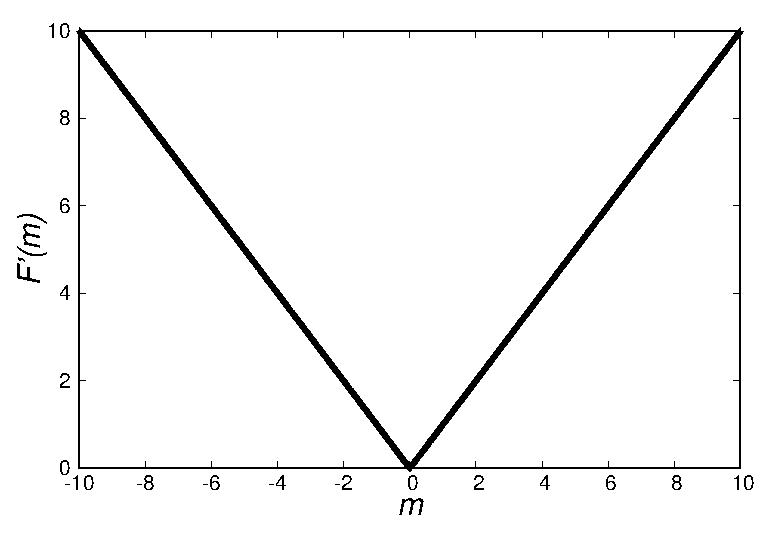
\includegraphics[keepaspectratio,scale=0.33]{minimum_cost.eps}
      \end{minipage}
      \begin{minipage}{0.50\hsize}
        \centering
        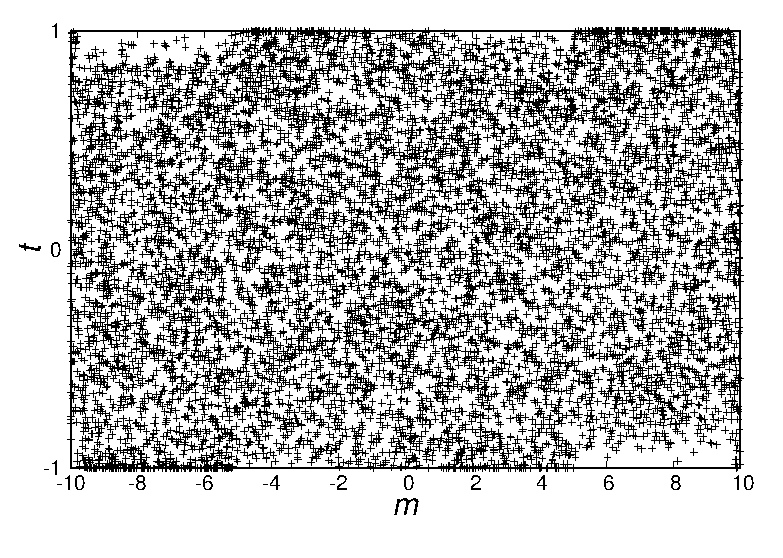
\includegraphics[keepaspectratio,scale=0.33]{minimum_t.eps}
      \end{minipage} \\
      \begin{minipage}{0.50\hsize}
        \centering
        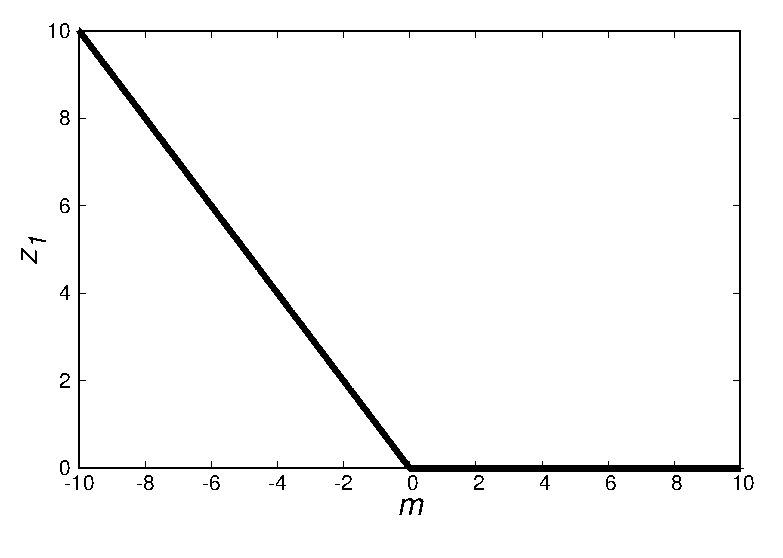
\includegraphics[keepaspectratio,scale=0.33]{minimum_z1.eps}
      \end{minipage}
      \begin{minipage}{0.50\hsize}
        \centering
        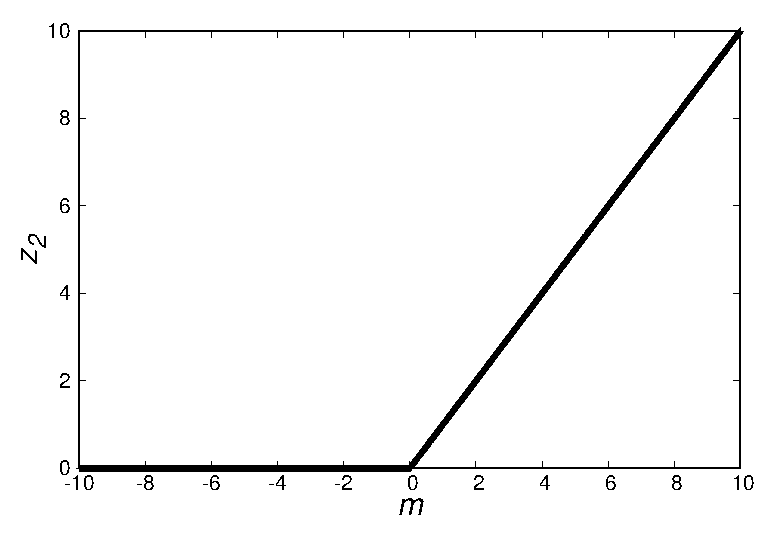
\includegraphics[keepaspectratio,scale=0.33]{minimum_z2.eps}
      \end{minipage}
    \end{tabular}
    \caption{The figures for upper left, upper right, lower left and lower right show the results when $\widetilde{F}(m), t, z_{1}, z_{2}$ are optimized for each $m$ respectively.}
    \label{fig:minimum1}
  \end{center}
\end{figure}

From this result, we can confirm that l1-norm can be obtained by optimizing (\ref{after_wolf}). Also, if we look at each variable $t, z_{1}$ and $z_{2}$ at optimization, we can see the following: It may be possible to reduce one variable by reviewing the (\ref{after_wolf}) because $t$ is not converged alothough $z_{1}$ and $z_{2}$ converge to a specific value.

\section{Reduced QUBO formulation} %定式化の見直し
\subsection{Reduction of the variable in the Legendre transformation}
We can think of the following from the results of the numerical experiments in the previous section: The variable $t$ seems to be taking a random value rather than settling to the optimal value, so we will consider whether we can eliminate $t$ by reviewing the formulation. 
The cost function can be transformed as follows using equality constraint.
\begin{alignat}{2}
  F'(m)&=\min_{t,z_{1},z_{2}}{\{mt+z_{1}(t+1)-z_{2}(t-1)} \nonumber \\
  &\quad+M(-m-z_{1}+z_{2})^{2}\} \nonumber \\
  &=\min_{t,z_{1},z_{2}}{\{mt+z_{1}(t+1)-(m+z_{1})(t-1)} \nonumber \\
  &\quad+M(-m-z_{1}+z_{2})^{2}\} \nonumber \\
  &=\min_{z_{1},z_{2}}{\{z_{1}+(m+z_{1})+M(-m-z_{1}+z_{2})^{2}\}} \nonumber \\
  &=\min_{z_{1},z_{2}}{\{z_{1}+z_{2}+M(-m-z_{1}+z_{2})^{2}\}} \label{review_formulation}
\end{alignat}
This conversion from (\ref{after_wolf}) to (\ref{review_formulation}) is possible because the penalty term, $M(-m-z_{1}+z_{2})^{2}$, forces the equality constraint to be satisfied.

\subsection{Numerical validation} %定式化したものを利用して実験を行う
The result of experimenting the optimization problem under the same experimental conditions as Section\ref{experiment_condition} with (\ref{review_formulation}) as the objective function is as shown in Fig.\ref{fig:minimum2}.
\begin{figure}[htbp]
  \begin{center}
    \begin{tabular}{c}
      \begin{minipage}{0.50\hsize}
        \centering
        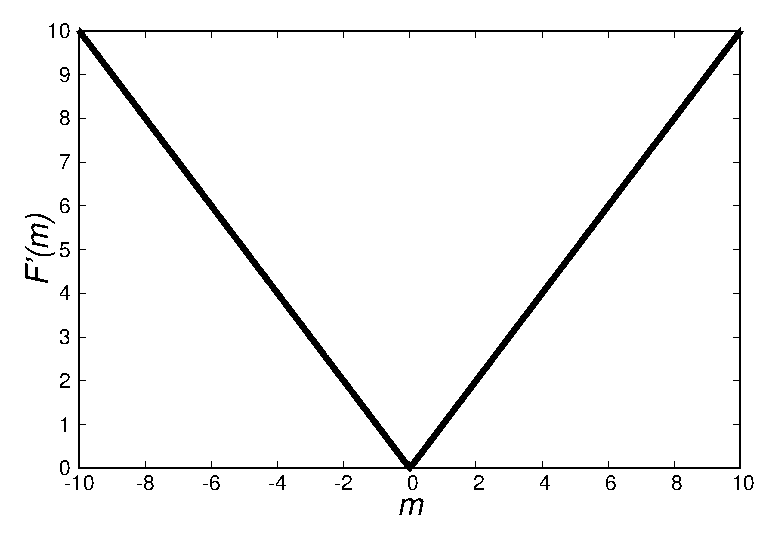
\includegraphics[keepaspectratio,scale=0.33]{minimum_cost_non_t.eps}
      \end{minipage} \\
      \begin{minipage}{0.50\hsize}
        \centering
        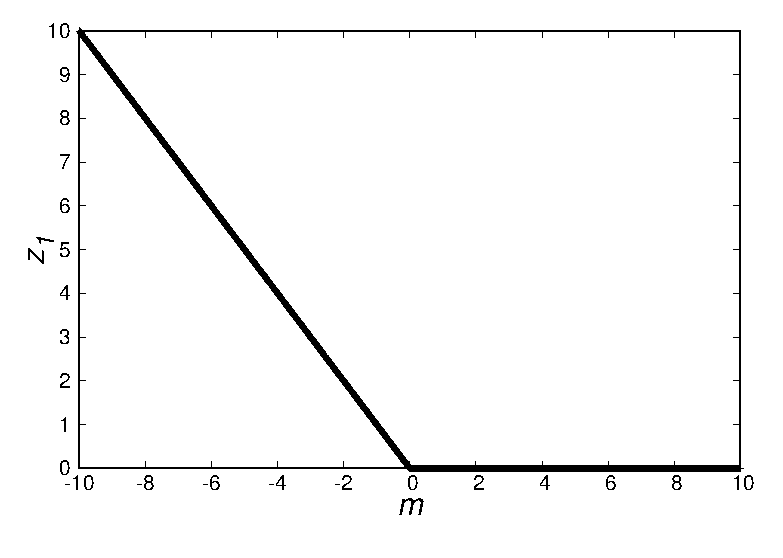
\includegraphics[keepaspectratio,scale=0.33]{minimum_z1_non_t.eps}
      \end{minipage}
      \begin{minipage}{0.50\hsize}
        \centering
        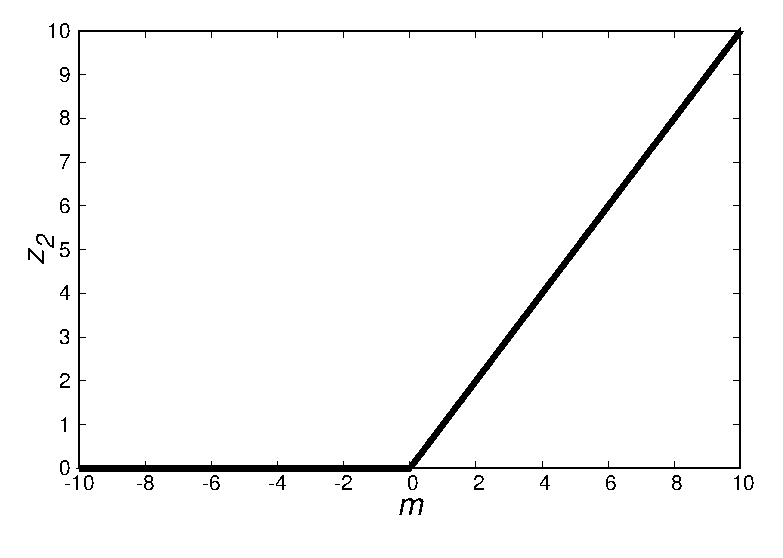
\includegraphics[keepaspectratio,scale=0.33]{minimum_z2_non_t.eps}
      \end{minipage}
    \end{tabular}
    \caption{The figures for upper, lower left and lower right show the results when $\widetilde{F}(m), z_{1}, z_{2}$ are optimized for each $m$ respectively.}
    \label{fig:minimum2}
  \end{center}
\end{figure}
From this result, the outline of $\widetilde{F}(m), z_{1}$ and $z_{2}$ when optimizing (\ref{after_wolf}) did not change from Fig.\ref{fig:minimum2}, so we seem that removing the variable $t$ does not affect the result.

\section{conclsion}


\begin{acknowledgment}

%\acknowledgment

%For enveironments for acknowledgment(s) are available: \verb|acknowledgment|, \verb|acknowledgments|, \verb|acknowledgment|, and \verb|acknowledgments|.

\end{acknowledgment}

%\appndix
%\section{}
%Use the \verb|\appendix| command if you need an appendix(es). The \verb|\section| command should follow even though there is no title for the appendix (see above in the source of this file).
%For authurs of Invited Review Papers, the \verb|profile| command si prepared for the author(s)' profile. A simple example is shown below.

%\begin{verbatim}
%\profile{Taro Butsuri}{was born in Tokyo, Japan in 1965. ...}
%\end{verbatim}

\begin{thebibliography}{1}
\bibitem{d-wave01}
  M. W. Johnson, M. H. S. Amin, S. Gildert, T. Lanting, F. Hamze, N. Dickson, R. Harris, A. J. Berkley, J. Johansson, P. Bunyk, E. M. Chapple, C. Enderud, J. P. Hilton, K. Karimi, E. Ladizinsky, N. Ladizinsky, T. Oh, I. Perminov, C. Rich, M. C. Thom, E. Tolkacheva, C. J. S. Truncik, S. Uchaikin, J. Wang, B. Wilson and G. Rose, Nature. {\bf 473}, 194 (2011).
\bibitem{d-wave02}
  P. I. Bunyk, E. Hoskinson, M. W. Johnson, E. Tolkacheva, F. Altomare, A. J. Berkley, R. Harris, J. P. Hilton, T. Lanting, J. Whittaker, IEEE Trans. Appl. Supercond. {\bf 24}, 1700110 (2014).
\bibitem{DA}
  M. Aramon, G. Rosenberg, E. Valiante, T. Miyazawa, H. Tamura, and H. G. Katzgraber, arXiv:1806.08815.
\bibitem{q-loss}
  V. Denchev, N.Ding, S. V. N Vishwanathan, and H. Neven, in Proceedings of the 29th International Conference on Machine Learning, p.863 (2012).
\bibitem{relu}
  Go Sato, Makiko Konoshima, Takuya Ohwa, Hirotaka Tamura and Jun Ohkubo, arXiv:1911.03829.
\bibitem{wolfe}
  P. Wolfe, Quart. Appl. Math. {\bf 19}, 239 (1961).
\bibitem{lasso}
  Robert Tibshirani, Regression Shrinkage and Selection via the Lasso, J. R. Statist. Soc, B, 58(1):267-288 (1996).
  
\end{thebibliography}

\end{document}

